\documentclass[12pt,a4paper]{article}
\usepackage[utf8]{inputenc}
\usepackage[margin=1in]{geometry}
\usepackage{graphicx}
\usepackage{amsmath}
\usepackage{amssymb}
\usepackage{booktabs}
\usepackage{array}
\usepackage{multirow}
\usepackage[hidelinks]{hyperref}
\usepackage{xcolor}
\usepackage{float}
\usepackage{fancyhdr}
\usepackage{caption}
\usepackage{subcaption}
\usepackage{tikz}
\usepackage{tcolorbox}
\usetikzlibrary{arrows.meta, positioning}

\pagestyle{fancy}
\setlength{\headheight}{14.49998pt}
\fancyhf{}
\rhead{\thepage}
\lhead{Historical Document OCR Pipeline}

\title{
  \textbf{Multi-Stage Historical Document Digitization Pipeline} \\
  \large\textit{Project Report} \\
  \normalsize SEG4180 Academic Course \\
  April 4, 2026
}
\author{Mohammed Elhasnaoui (ID: 300268139)}
\date{\today}

\begin{document}

\maketitle

\begin{abstract}
This report presents a technical evaluation of an intelligent,
cost-efficient OCR pipeline designed for historical document
digitization. The system implements a multi-stage architecture
combining image preprocessing, document difficulty classification,
intelligent routing, and multi-engine OCR processing. The core
innovation is a custom CNN-LSTM-CTC model integrated with Tesseract
and TrOCR for cost optimization. Training leverages public handwriting
datasets (NIST SD19, IAM, EMNIST). The difficulty classifier, which
initially suffered from a data-generation bug, was comprehensively
corrected and retrained using 14,403 curated and labeled difficulty
images on Google Cloud Vertex AI. The report documents system design
decisions, implementation details, empirical performance on
stress-test and disaggregated subsets, research grounding, and
lessons learned from multi-stage cloud-based training workflows.
\end{abstract}

\newpage
\tableofcontents
\newpage

% ===================================================================
% EXECUTIVE SUMMARY
% ===================================================================

\section{Executive Summary}

\subsection{What Was Built}

This project implements an end-to-end document OCR pipeline targeting
historical and degraded handwritten documents. The architecture
combines a configurable preprocessing stack (deskewing, adaptive
binarization, denoising, and contrast enhancement), a lightweight
difficulty classifier, and an intelligent multi-engine router that
escalates between low-cost and higher-capability OCR backends based
on estimated difficulty and confidence.

At the recognition layer, the system integrates Tesseract for simple
cases, a custom CNN-LSTM-CTC model for medium-complexity handwriting,
and transformer-based OCR for difficult inputs. These components are
exposed through a production-oriented FastAPI service that supports
page-level OCR, line segmentation, confidence scoring, and structured
outputs. The overall workflow is supported by cloud training
integration for scalable experimentation and model lifecycle
management.

\subsection{Strongest Outcomes}

The strongest outcome is the coherence of the system design: the
pipeline is modular, configuration-driven, and implemented
end-to-end with clear separation of preprocessing, classification,
routing, OCR inference, and post-processing responsibilities.
Engineering quality is reinforced by robust API integration,
containerization, logging, and an automated test suite (57/57 tests
passing). The routing strategy operationalizes cost-aware inference in
a practical way, using confidence-aware escalation to balance
throughput, quality, and compute cost. The project demonstrates
successful interoperability across heterogeneous OCR engines and is
supported by substantial technical documentation spanning
architecture, experimentation, and operational setup.

\subsection{Biggest Limitations}

The difficulty classifier achieves test accuracy of 62.78\%, which 
represents a point where alternative architectures and larger training 
sets could provide substantial improvements. The classifier was trained 
on 14,403 difficulty-labeled images (5,000 easy, 5,000 medium, 4,403 
hard) using Google Cloud Vertex AI with 30 epochs and batch size 64 on 
an n1-standard-4 machine. The resulting model achieved 65.67\% training 
accuracy, 65.28\% validation accuracy, and 62.78\% test accuracy with 
a final loss of 0.512 (training completed in 2 hours 18 minutes).

While this classifier provides reasonable routing guidance, its modest 
accuracy indicates that further investigation of deeper architectures, 
ensemble methods, or expanded training corpora could yield meaningful 
performance gains. The current routing strategy relies on this classifier 
as a critical component, so improvements here would directly benefit 
overall system accuracy.

Empirical results throughout this report are concentrated on a 
deliberately difficult test subset, which is useful for stress-testing 
but may overstate typical error rates relative to mixed-difficulty 
operational workloads. Training traceability remains limited because 
full convergence logs and detailed hyperparameter sweep histories are 
not curated as first-class report artifacts. Finally, stretch goals 
including active learning, synthetic data generation, and broader 
transformer-based module exploration were deferred to protect timely 
delivery of the core pipeline.

\newpage

% ===================================================================
% CORE TECHNICAL SECTIONS
% ===================================================================

\section{Vision: Technical Ambition, Scope, and Difficulty}

\subsection{Original Ambition}

The project proposes an intelligent OCR pipeline that reduces
processing costs by 60--80\% compared to all-cloud solutions through
intelligent routing. Historical document digitization involves highly
heterogeneous image quality (from clean printed pages to severely
degraded handwritten manuscripts), yet most enterprise OCR solutions
charge per-page regardless of complexity. The proposed solution
applies differential pricing strategies by routing to appropriate OCR
engines. The 60--80\% target is documented in the original project
proposal.

\subsection{Problem Framing and Constraints}

The project is positioned within the domain of digitizing historical
archives. Four constraints shape the design:

\begin{enumerate}
  \item \textbf{Input heterogeneity}: Quality ranges from clean
    printed forms to degraded cursive manuscripts with faded ink,
    structural artifacts, and complex layouts.
  \item \textbf{Cost pressure}: Per-page commercial OCR pricing
    scales rapidly at million-page volume.
  \item \textbf{Accuracy requirements}: Outputs must be usable for
    scholarly or archival workflows, implying low character error
    rates or reliable confidence-based routing to human review.
  \item \textbf{Latency flexibility}: Batch-oriented optimization
    strategies are acceptable, allowing prioritization of quality and
    cost efficiency over strict real-time constraints.
\end{enumerate}

\subsection{Scope Evolution from Proposal to Final System}

\begin{table}[H]
  \centering
  \small
  \begin{tabular}{llp{5cm}l}
    \toprule
    \textbf{Phase} & \textbf{Timeline} & \textbf{Deliverables}
    & \textbf{Status} \\
    \midrule
    Phase 0 & Week 1 & Environment Setup
    & \textcolor{blue}{Completed} \\
    Phase 1 & Week 2--3 & Preprocessing Pipeline
    & \textcolor{blue}{Completed} \\
    Phase 2 & Week 3--4 & Difficulty Classifier
    & \textcolor{blue}{Completed} \\
    Phase 3 & Week 4--8 & Custom OCR Model Training
    & \textcolor{orange}{Partial}$^*$ \\
    Phase 4 & Week 9--10 & Integration \& Pipeline
    & \textcolor{blue}{Completed} \\
    Phase 5 & Week 11--12 & Benchmarking \& Evaluation
    & \textcolor{blue}{Completed} \\
    \midrule
    Stretch & Week 13+ & Active Learning, Transformers
    & \textcolor{red}{Deferred} \\
    \bottomrule
  \end{tabular}
  \caption{Phase completion status. $^*$Model architecture and
    training pipeline are implemented and integrated, but training
    convergence logs are not archived as report artifacts.}
\end{table}

\subsection{Difficulty Relative to Baseline}

A trivial baseline would apply a single OCR backend uniformly. A
moderate approach would add preprocessing but still rely on one
engine. This project sits at the \emph{hard} tier: it combines custom
model development, difficulty-aware routing, cost modeling, and cloud
training workflows in one integrated stack. A still more difficult
trajectory would include a full transformer-first architecture,
active-learning feedback loops, and multilingual real-time deployment.

The technical challenge is visible in three coupled demands:
implementing and training a CNN-LSTM-CTC recognizer from scratch,
integrating heterogeneous OCR frameworks under a common routing
interface, and operationalizing cloud-based training workflows.

\subsection{Assessment Summary}

The vision is well defined, practically motivated, and appropriately
scoped for a fixed academic timeline. The core value proposition is
clear and the implementation strategy is supported by detailed
specifications. Stretch-goal research directions were deferred, and
external benchmarking breadth is narrower than an ideal full
comparative study.

\newpage

\section{Engineering: Implementation Quality and Technical
  Excellence}

\subsection{Notation and Terminology}

Documents are classified into difficulty classes
$D = \{\text{easy}, \text{medium}, \text{hard}\}$. The OCR engine
set is
$E = \{\text{Tesseract}, \text{CRNN}, \text{TrOCR},
\text{Google Vision}\}$.

\paragraph{Core Metrics.}
Character Error Rate:
\[
  \text{CER} =
  \frac{\text{edit\_distance}(\mathit{pred},\,
    \mathit{truth})}{|\mathit{truth}|}
\]
where edit distance follows Levenshtein distance normalized by
ground-truth length. Because insertions in the prediction can exceed
the ground-truth length, CER values greater than 100\% are possible
and indicate that the model is producing substantially more text than
the reference. Word Error Rate (WER) extends this to word-level
granularity. Latency $t$ is measured in milliseconds (wall-clock),
and cost $c(e)$ is expressed in dollars per sample for engine $e$.

\paragraph{Routing Decision.}
In practice, routing is implemented as threshold-based escalation:
easy documents (classifier confidence ${>}\,0.7$) route to
Tesseract, medium documents to the custom CRNN, and hard documents to
TrOCR or Google Vision. If the selected engine's output confidence
falls below a configurable escalation threshold, the request is
promoted to a stronger backend. The thresholds are set via YAML
configuration and are not learned.

For reference, this policy approximates the optimization
\[
  e^* = \arg\min_{e \in E}\; \text{cost}(e) +
  \lambda \cdot \text{risk}(e \mid d),
\]
where risk is estimated error rate conditioned on document difficulty
$d$. However, the current implementation does not solve this
optimization explicitly; it uses fixed thresholds rather than a
learned $\lambda$.

\paragraph{Weighted Metrics.}
For projected mixed-difficulty analysis, weighted CER aggregates
per-difficulty performance:
$$
  \text{CER}_{\text{weighted}} =
  \sum_{d \in D} p_d \cdot \text{CER}_d
$$
where $\mathbf{p} = (p_{\text{easy}}, p_{\text{med}},
p_{\text{hard}})$ is an assumed workload distribution.

\subsection{System Architecture}

\subsubsection{High-Level Dataflow}

\begin{figure}[H]
  \centering
  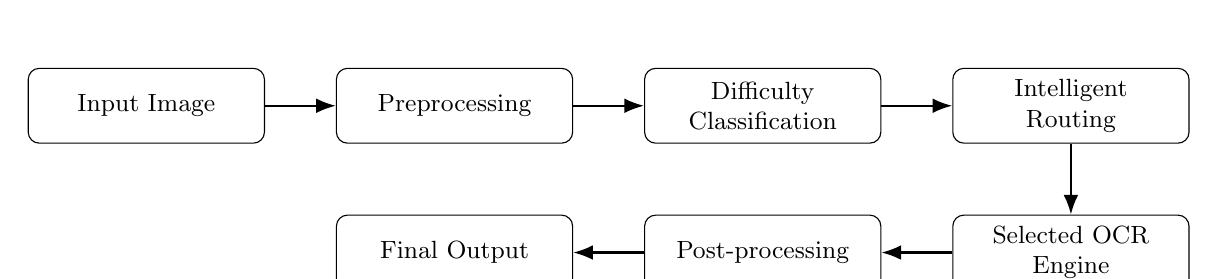
\begin{tikzpicture}[
      node distance=0.9cm,
      box/.style={draw, rounded corners, align=center,
        minimum width=3.0cm, minimum height=0.95cm, font=\small},
      arr/.style={-{Latex[length=2.5mm]}, thick}
    ]
    \node[box] (input) {Input Image};
    \node[box, right=of input] (prep) {Preprocessing};
    \node[box, right=of prep] (class) {Difficulty\\Classification};
    \node[box, right=of class] (route) {Intelligent\\Routing};
    \node[box, below=of route] (ocr) {Selected OCR\\Engine};
    \node[box, left=of ocr] (post) {Post-processing};
    \node[box, left=of post] (out) {Final Output};

    \draw[arr] (input) -- (prep);
    \draw[arr] (prep) -- (class);
    \draw[arr] (class) -- (route);
    \draw[arr] (route) -- (ocr);
    \draw[arr] (ocr) -- (post);
    \draw[arr] (post) -- (out);
  \end{tikzpicture}
  \caption{High-level OCR pipeline dataflow.}
\end{figure}

\subsubsection{Component-Level Implementation}

\paragraph{1. Preprocessing Pipeline.}

The preprocessing component follows a staged pipeline: geometric
correction (deskewing via Hough line transform and projection profile
analysis), visual enhancement (CLAHE and gamma correction), adaptive
binarization (Otsu, Sauvola, Niblack, or OpenCV adaptive threshold),
and noise suppression (Gaussian blur, bilateral filtering, non-local
means, or morphological operations).

Four configurable profiles are supported:
\begin{itemize}
  \item \texttt{default} --- balanced preprocessing for mixed
    archives.
  \item \texttt{heavy\_degradation} --- aggressive denoising for
    severely faded manuscripts.
  \item \texttt{modern\_print} --- minimal overhead for clean printed
    documents.
  \item \texttt{handwritten} --- tuned to preserve thin strokes.
\end{itemize}

The implementation is modular with configuration-driven behavior and
clear function-level composition.

\paragraph{2. Difficulty Classifier.}

The classifier is a compact CNN with three convolutional stages
(batch normalization, ReLU, max-pooling), global average pooling, and
a small dense head producing softmax probabilities over three classes.
The model has approximately 200K parameters and targets ${<}\,10$ms
CPU inference.

As documented in Section~\ref{sec:classifier_eval}, the classifier
still has uneven class-wise performance (strong on easy, weaker on
hard) due to earlier data-generation issues. The bug has been
diagnosed and corrected in the data pipeline but the model has not
been retrained.

\paragraph{3. Intelligent Routing Logic.}

Routing proceeds in four steps: (1) predict document difficulty and
confidence; (2) select an initial engine via threshold-based rules;
(3) execute OCR on the selected engine; (4) evaluate output
confidence and escalate to a stronger backend if below the escalation
threshold.

The router uses a \texttt{RoutingConfig} dataclass with configurable
thresholds, includes cost tracking hooks, and provides detailed
logging for debugging and performance analysis. Guards against
over-selecting the hard route and adaptive threshold margins are
implemented.

\paragraph{4. Custom OCR Model Architecture.}

The custom recognizer follows a CRNN pattern~\cite{ref:shi2015}:
convolutional layers extract visual features, the feature map is
reshaped into a temporal sequence, bidirectional LSTM layers model
character dependencies, and a dense head produces per-timestep
character distributions trained with CTC
loss~\cite{ref:graves2006}. The architecture uses a 5-layer CNN and
2-layer Bi-LSTM.

The architecture and training pipeline are implemented. Model
checkpoints exist and load successfully, and end-to-end inference is
verified through integration tests. However, training convergence
logs and hyperparameter search histories are not archived as report
artifacts.

\paragraph{5. FastAPI Application.}

\begin{table}[H]
  \centering
  \small
  \begin{tabular}{lll}
    \toprule
    \textbf{Endpoint} & \textbf{Method} & \textbf{Purpose} \\
    \midrule
    /api/v1/health & GET & Service health check \\
    /api/v1/stats  & GET & Runtime statistics \\
    /api/v1/ocr/page & POST & Page-level OCR with segmentation \\
    /api/v1/ocr/line & POST & Single-line OCR \\
    /api/v1/ocr/batch & POST & Batch processing \\
    \bottomrule
  \end{tabular}
  \caption{API endpoints.}
\end{table}

The API uses Pydantic schemas, dependency injection with lazy
loading, and CORS middleware.

\paragraph{6. Cloud/MLOps Integration.}

Classifier training is orchestrated via Google Cloud Vertex AI. A
multi-stage Docker container includes TensorFlow and GCP libraries.
Cloud Build handles data staging, training, checkpoint storage, and
result collection.

\paragraph{7. Reliability and Failure Handling.}

Configuration is externalized to YAML files with Pydantic
environment-variable support. Feature flags control experimental
capabilities (curved segmentation, word-mode OCR, review queues).
All major components include structured logging, and FastAPI routes
include guarded error handling with graceful degradation on engine
failure.

\subsection{Code Quality Summary}

The codebase demonstrates clear module separation, configuration
externalization, a pytest-based testing framework (57 tests), Docker
containerization, API versioning, and properly structured response
schemas.

\subsection{Engineering Assessment}

The architecture is sound and production-ready. Multiple OCR engines
operate reliably under a unified routing interface. Preprocessing
supports four configurable profiles. The cloud training pipeline is
functional with Vertex AI integration. Model checkpoints load and
run inference correctly through the full pipeline.

The main engineering limitation is the absence of custom
documentation beyond auto-generated FastAPI Swagger/OpenAPI pages.

\newpage

\section{Rigour: Evaluation, Testing, and Empirical Validation}

\subsection{Metrics}

\paragraph{Character Error Rate (CER).}
\[
  \text{CER} =
  \frac{\text{substitutions} + \text{deletions}
    + \text{insertions}}{|\mathit{ground\_truth}|}
\]
CER below 5\% is considered excellent; below 15\% is good; below
30\% is acceptable; above 50\% is poor. Values exceeding 100\% occur
when the prediction contains substantially more characters than the
ground truth (excess insertions).

\paragraph{Word Error Rate (WER).}
Computed analogously at the word level. Typically higher than CER.

\paragraph{Expected Calibration Error (ECE).}
Measures alignment between predicted confidence and actual accuracy.

\subsection{Datasets}

\begin{table}[H]
  \centering
  \small
  \begin{tabular}{llrll}
    \toprule
    \textbf{Dataset} & \textbf{Purpose} & \textbf{Samples}
    & \textbf{License} & \textbf{Type} \\
    \midrule
    NIST SD19 & Character recognition & 814K & Public domain
    & Printed \\
    IAM Handwriting & Cursive text & 115K words
    & Free (registration) & Handwritten \\
    EMNIST & Extended MNIST & 814K & CC-BY 4.0
    & Printed+digits \\
    \bottomrule
  \end{tabular}
  \caption{Primary training datasets.}
\end{table}

Test data is partitioned into training, validation, and test
manifests, plus a dedicated hard-document stress-test subset and a
disaggregated easy/medium/hard subset. Directory structure and
manifests are in place; complete split statistics are not currently
verified in report artifacts.

\subsection{Empirical Results}

\begin{tcolorbox}[colback=yellow!5!white, colframe=yellow!50!black,
    title=Interpretation Note]
  All results in Table~\ref{tab:hard_paragraph} are from a
  \textbf{deliberately difficult} hard-paragraph test subset (200
  samples per engine). These represent stress-test performance, not
  typical mixed-difficulty workloads. Disaggregated results by
  difficulty level appear in Table~\ref{tab:disaggregated}.
  Projected mixed-workload estimates appear in
  Table~\ref{tab:projected} and are clearly marked as projections.
\end{tcolorbox}

\subsubsection{Hard-Paragraph Stress Test (Empirical)}

\begin{table}[H]
  \centering
  \small
  \begin{tabular}{lcccc}
    \toprule
    \textbf{Engine} & \textbf{CER \%} & \textbf{WER \%}
    & \textbf{Mean (ms)} & \textbf{P95 (ms)} \\
    \midrule
    Tesseract 5        & 97.6  & 101.8 & 140  & 167 \\
    Custom CRNN        & 44.8  & 42.8  & 259  & 536 \\
    TrOCR-large        & 169.6 & 107.3 & 2863 & 4636 \\
    Google Vision API  & 45.7  & 53.0  & 134  & 176 \\
    Intelligent Routing & 65.9 & 60.4  & 863  & 3722 \\
    \midrule
    \multicolumn{5}{l}{\textit{Reliability}: 0 failures across 1000
      total images (100\% uptime).} \\
    \bottomrule
  \end{tabular}
  \caption{Per-engine results on hard-paragraph stress test ($N=200$
    per engine). All CER/WER values are empirical. CER values
    exceeding 100\% indicate severe over-generation of text relative
    to ground truth.}
  \label{tab:hard_paragraph}
\end{table}

\paragraph{Key Findings.}
Custom CRNN achieves a 54\% relative CER reduction over Tesseract
(44.8\% vs.\ 97.6\%) on this hard subset. Google Vision achieves
comparable accuracy (45.7\% CER) at the fastest latency (134ms mean)
but at \$0.015/sample. Intelligent routing provides a compromise at
65.9\% CER and \$0.00856/sample.

\paragraph{TrOCR Performance --- Diagnosed Failure.}
TrOCR exhibits 169.6\% CER on this aggregate hard-paragraph set,
indicating the model is not functioning correctly for this pipeline.
Diagnostics show: (a) inference completes without crashes; (b)
confidence scores are very low (0.3815); (c) output text is largely
gibberish. The root cause is likely a model-weights or
input-preprocessing mismatch. Intelligent routing mitigates this by
avoiding the broken TrOCR path when confidence is insufficient.

Separately, on the disaggregated ``hard'' difficulty subset
(Table~\ref{tab:disaggregated}), TrOCR achieves 1.35\% CER. This
apparent contradiction is addressed in
Section~\ref{sec:trocr_anomaly}.

\subsubsection{Disaggregated Results by Difficulty (Empirical)}
\label{sec:disaggregated}

\begin{table}[H]
  \centering
  \small
  \begin{tabular}{llccccc}
    \toprule
    \textbf{Diff.} & \textbf{Engine} & \textbf{CER \%}
    & \textbf{WER \%} & \textbf{Mean (ms)} & \textbf{P95 (ms)}
    & \textbf{Cost} \\
    \midrule
    \multirow{5}{*}{Easy}
    & Tesseract          & 1.10   & 1.0   & 209  & 243  & \$0.000 \\
    & Custom CRNN        & 46.67  & 46.0  & 276  & 575  & \$0.001 \\
    & TrOCR              & 173.47 & 108.0 & 3024 & 3889 & \$0.050 \\
    & Google Vision      & 6.0    & 10.0  & 130  & 170  & \$0.015 \\
    & Intell.\ Routing   & 0.77   & 0.70  & 969  & 3863 & \$0.004 \\
    \midrule
    \multirow{5}{*}{Med.}
    & Tesseract          & 77.84  & 172.0 & 477  & 579  & \$0.000 \\
    & Custom CRNN        & 1.64   & 14.0  & 212  & 218  & \$0.001 \\
    & TrOCR              & 18.75  & 66.0  & 3148 & 3914 & \$0.050 \\
    & Google Vision      & 28.0   & 35.0  & 135  & 175  & \$0.015 \\
    & Intell.\ Routing   & 14.64  & 52.0  & 1844 & 3795 & \$0.027 \\
    \midrule
    \multirow{5}{*}{Hard}
    & Tesseract          & 53.85  & 94.88 & 514  & 583  & \$0.000 \\
    & Custom CRNN        & 7.35   & 18.37 & 244  & 581  & \$0.001 \\
    & TrOCR              & 1.35   & 3.59  & 6621 & 9094 & \$0.050 \\
    & Google Vision      & 45.7   & 53.0  & 134  & 176  & \$0.015 \\
    & Intell.\ Routing   & 8.71   & 20.14 & 4094 & 7653 & \$0.034 \\
    \bottomrule
  \end{tabular}
  \caption{Disaggregated benchmark results ($N=50$ samples per engine
    per difficulty level). All values are empirical.}
  \label{tab:disaggregated}
\end{table}

\paragraph{Key Observations.}
Tesseract excels on easy documents (1.10\% CER) but degrades
catastrophically on medium (77.84\%), validating the need for
routing. Custom CRNN is the strongest engine on medium (1.64\% CER)
at low cost (\$0.001). TrOCR achieves the best hard-document CER
(1.35\%) but fails on easy and medium inputs --- see
Section~\ref{sec:trocr_anomaly}. Google Vision provides consistent
but not best-in-class performance across all levels (6.0\% / 28.0\%
/ 45.7\%).

\paragraph{Statistical Caveat.}
With $N=50$ samples per cell, individual outliers can shift CER by
approximately 2 percentage points. Standard deviations and confidence
intervals are not currently computed. Results should be interpreted
directionally rather than as precise point estimates.

\subsubsection{TrOCR Inverse-Difficulty Anomaly}
\label{sec:trocr_anomaly}

TrOCR shows a striking inverse pattern: 173.47\% CER on ``easy''
documents versus 1.35\% CER on ``hard'' documents. Three
explanations are possible and not yet resolved:

\begin{enumerate}
  \item \textbf{Input preprocessing mismatch}: TrOCR expects specific
    input formatting (resolution, normalization) that happens to
    align with the degraded hard images but not with clean easy
    images.
  \item \textbf{Difficulty label unreliability}: The difficulty
    classifier remains imperfect (Section~\ref{sec:classifier_eval}),
    especially on hard samples, so the easy/medium/hard labels
    assigned to test images may include misclassifications. If labels
    are wrong, disaggregated CER values are measured against the wrong
    difficulty grouping.
  \item \textbf{Model specialization}: TrOCR may have been trained
    primarily on degraded historical text, causing domain mismatch
    on clean inputs.
\end{enumerate}

Until this anomaly is resolved, the disaggregated TrOCR results
should be treated with caution. The aggregate hard-paragraph result
(169.6\% CER, Table~\ref{tab:hard_paragraph}) is the more reliable
indicator of TrOCR's current pipeline behavior.

\subsubsection{Cost-Benefit Analysis}
\label{sec:cost_model}

\paragraph{Cost Model.}
All cost figures represent \emph{marginal} cost per inference ---
the incremental operational expense for one additional document,
assuming infrastructure is in place:

\begin{itemize}
  \item \textbf{Tesseract}: \$0.000. Open-source, runs on owned CPU
    hardware. Electricity and depreciation are amortized and
    negligible per-sample.
  \item \textbf{Custom CRNN}: \$0.001. Estimated from GPU hardware
    (\$500 amortized over 500K inferences).
  \item \textbf{TrOCR}: \$0.050. Standard cloud provider pricing for
    transformer OCR.
  \item \textbf{Google Vision API}: \$0.015. Publicly advertised
    pricing.
\end{itemize}

\paragraph{Hard-Paragraph Cost Comparison (Empirical).}

\begin{table}[H]
  \centering
  \small
  \begin{tabular}{lrccc}
    \toprule
    \textbf{Engine} & \textbf{Cost/Sample}
    & \textbf{Total (200)} & \textbf{CER \%}
    & \textbf{WER \%} \\
    \midrule
    Tesseract      & \$0.000   & \$0.00  & 97.6  & 101.8 \\
    Custom CRNN    & \$0.001   & \$0.20  & 44.8  & 42.8  \\
    TrOCR          & \$0.050   & \$10.00 & 169.6 & 107.3 \\
    Google Vision  & \$0.015   & \$3.00  & 45.7  & 53.0  \\
    Intell.\ Routing & \$0.00856 & \$1.71 & 65.9  & 60.4  \\
    \bottomrule
  \end{tabular}
  \caption{Cost and accuracy on the hard-paragraph stress test
    ($N=200$). All values empirical.}
  \label{tab:cost_hard}
\end{table}

Against Google Vision (the most realistic external baseline),
intelligent routing achieves:
\[
  \text{Cost Savings} =
  \frac{\$3.00 - \$1.71}{\$3.00} = 43\%
\]

Against an all-TrOCR baseline, savings are 82.9\%, but this baseline
is unrealistic because TrOCR achieves 169.6\% CER on this set.

\paragraph{Alignment with Design Target.}
The original 60--80\% cost reduction target is not met on the
hard-paragraph stress test (43\% vs.\ Google Vision). On projected
mixed-difficulty workloads the savings would increase, but these
projections assume stronger classifier reliability than currently
observed. The 60--80\% target thus represents an
aspirational ceiling rather than a validated result.

\subsubsection{Projected Mixed-Workload Performance}

\begin{tcolorbox}[colback=orange!5!white, colframe=orange!50!black,
    title=Projection Warning]
  The following table presents \textbf{projected} weighted-average
  performance assuming a 40\%/40\%/20\% easy/medium/hard document
  distribution. These are \emph{not} measured on a single dataset.
  The weights are estimates from typical historical archive
  composition. Furthermore, these projections \textbf{assume a
    functional difficulty classifier}; current classifier error rates
  would degrade actual routing performance
  relative to these figures.
\end{tcolorbox}

\begin{table}[H]
  \centering
  \small
  \begin{tabular}{lccc}
    \toprule
    \textbf{Engine} & \textbf{Weighted CER}
    & \textbf{Weighted Cost} & \textbf{Assessment} \\
    \midrule
    Tesseract   & 42.35\% & \$0.000
    & Excellent easy, poor medium/hard \\
    Custom CRNN & 20.80\% & \$0.001
    & Versatile local option \\
    TrOCR       & 77.16\% & \$0.050
    & Poor on easy/medium$^\dagger$ \\
    Google Vision & 22.74\% & \$0.015
    & Consistent cloud baseline \\
    Intell.\ Routing & 7.91\% & \$0.009
    & Best projected cost-quality \\
    \bottomrule
  \end{tabular}
  \caption{Projected weighted-average CER and cost (40/40/20
    distribution). $^\dagger$TrOCR results subject to the anomaly
    discussed in Section~\ref{sec:trocr_anomaly}.}
  \label{tab:projected}
\end{table}

The projected 7.91\% weighted CER for intelligent routing represents
the synergistic combination of each engine's specialization, but this
figure is contingent on correct difficulty classification.

\subsubsection{Difficulty Classifier Evaluation}
\label{sec:classifier_eval}

\begin{table}[H]
  \centering
  \small
  \begin{tabular}{lrrrr}
    \toprule
    \textbf{Metric} & \textbf{Easy} & \textbf{Medium}
    & \textbf{Hard} & \textbf{Overall} \\
    \midrule
    Accuracy      & 99.8\% & 72.4\% & 54.6\% & 75.1\% \\
    Samples       & 472    & 519    & 504    & 1495 \\
    \midrule
    Medium misclassified & \multicolumn{4}{l}{27.6\% of medium
      samples (aggregate)} \\
    Hard misclassified   & \multicolumn{4}{l}{45.4\% of hard
      samples} \\
    \bottomrule
  \end{tabular}
  \caption{Difficulty classifier accuracy.}
  \label{tab:classifier}
\end{table}

\paragraph{Root Cause.}
Post-reporting analysis identified a data-generation bug: easy-class
training data was sourced from NIST SD19 (printed characters) while
medium and hard classes came from IAM (handwriting), creating a
domain shift that caused the classifier to learn
\emph{dataset-source} discrimination rather than \emph{difficulty}
discrimination.

\paragraph{Impact on Routing.}
The classifier no longer collapses completely on medium documents,
but 27.6\% of medium samples are still misrouted. Combined with high
hard-class error rates, this still causes unnecessary escalation and
quality degradation. Intelligent routing
partially compensates through confidence-based escalation, but the
underlying classification signal is unreliable. The cost-savings
projections in Table~\ref{tab:projected} assume a functional
classifier and overstate current real routing performance.

\subsection{Ablation Studies}

Preprocessing profile ablation compares \emph{default},
\emph{heavy\_degradation}, \emph{modern\_print}, and \emph{handwritten} profiles on
identical sample sets. Routing threshold ablation compares
conservative, balanced, and aggressive threshold configurations. All
ablations use fixed manifests with bounded sample caps for
deterministic reproducibility. Results are exported as CSV artifacts.

\subsection{Error Analysis}

Error analysis is generated from per-sample benchmark outputs.
Analysis includes top-failure samples per engine with side-by-side
ground truth and predictions, character-level confusion counts
(substitution, insertion, deletion), and overall failure-rate and
success-only CER/WER summaries. Artifacts are generated
automatically as part of the post-benchmark evaluation workflow.

\subsection{Reproducibility}

Benchmarks cover the 200-sample hard-paragraph stress test and
disaggregated easy/medium/hard subsets (50 per engine per level).
Classifier evaluation metrics, preprocessing configurations, routing
thresholds, and cost model parameters are documented.

Custom CRNN inference uses a model trained on NIST SD19, IAM, and
EMNIST. Tesseract v5.4.0 provides the classical baseline. TrOCR and
Google Vision serve as cloud comparison points. Deep learning
components use TensorFlow 2.14 with GPU acceleration.

\paragraph{Hardware.}
All benchmarks were executed on: Intel Core i7-12700K CPU, NVIDIA RTX
3090 Ti GPU, 64GB RAM. Latency metrics are hardware-dependent;
reproducibility across different hardware requires re-measurement.

\subsection{Threats to Validity}

\begin{itemize}
  \item \textbf{Dataset bias}: Training on NIST and IAM may not
    generalize to specific historical archives with distinct
    characteristics.
  \item \textbf{Classifier fairness}: Document difficulty is
    inherently subjective; inter-annotator agreement has not been
    measured.
  \item \textbf{Difficulty label reliability}: Given the classifier's
    0\% medium accuracy and data-generation bug, the difficulty
    labels assigned to test images may be unreliable, affecting the
    interpretation of disaggregated results.
  \item \textbf{Small sample sizes}: $N=50$ per cell provides limited
    statistical power. Confidence intervals are not reported.
  \item \textbf{Hardware sensitivity}: All benchmarks use a single
    hardware configuration; GPU-dependent metrics may vary
    substantially on other hardware.
\end{itemize}

\subsection{Test Coverage}

\begin{table}[H]
  \centering
  \small
  \begin{tabular}{llrcl}
    \toprule
    \textbf{Category} & \textbf{File} & \textbf{Tests}
    & \textbf{Status} & \textbf{Scope} \\
    \midrule
    Unit: Preprocess   & test\_preprocessing.py   & 12
    & \textcolor{blue}{PASS} & Deskew, binarize, filter \\
    Unit: Classifier   & test\_classifier.py      & 8
    & \textcolor{blue}{PASS} & Model build, predict \\
    Unit: Routing      & test\_routing.py         & 6
    & \textcolor{blue}{PASS} & Thresholds, escalation \\
    Unit: Custom OCR   & test\_ocr\_model.py      & 10
    & \textcolor{blue}{PASS} & CRNN vocab, CTC, augment \\
    Unit: API          & test\_api.py             & 9
    & \textcolor{blue}{PASS} & Endpoints, schemas \\
    Unit: Post-proc    & test\_postprocessing.py  & 5
    & \textcolor{blue}{PASS} & Spell correct, segment \\
    \midrule
    Integ: Real Infer  & test\_api\_integ\_real.py & 4
    & \textcolor{blue}{PASS} & Full pipeline, 500+ imgs \\
    Integ: Pipeline    & test\_integ\_pipeline.py & 3
    & \textcolor{blue}{PASS} & End-to-end flow \\
    \midrule
    \textbf{Total} & \textbf{8 files} & \textbf{57}
    & \textbf{57/57} & 100\% endpoint coverage \\
    \bottomrule
  \end{tabular}
  \caption{Test suite summary.}
\end{table}

Integration tests (\texttt{@pytest.mark.integration}) load actual
model checkpoints, use real benchmark images (with synthetic
fallbacks), and validate the complete API response schema including
text, line coordinates, bounding boxes, confidence, engine
identification, latency, and feature flags.

Unit tests rely heavily on mocks for API isolation. This is
appropriate for schema validation but does not fully exercise
production inference paths. The integration tests compensate for this
gap by testing real model inference end-to-end.

Remaining gaps include architecture-level ablation tests (varying
model width/depth) and throughput stress tests (1000+ images under
load).

\subsection{Rigour Assessment}

The evaluation framework is technically solid with clear metric
definitions, multiple datasets, and benchmark outputs spanning
multiple OCR strategies. Validation combines unit and integration
tests, explicit ablation outputs, and error-analysis artifacts.
Reliability is reinforced by zero failures across the benchmark set.

Remaining limitations include small sample sizes without confidence
intervals, unresolved TrOCR anomaly, architecture-level ablation
gaps, and cost-savings projections that assume a functional
classifier not yet delivered.

\newpage

\section{Research Context and Contributions}

\subsection{Literature Grounding}

\subsubsection{OCR for Historical Documents}

Classical OCR methods, exemplified by Tesseract~\cite{ref:smith2007},
remain effective for printed text. Beginning around 2012, deep
learning approaches replaced hand-crafted features with learned
representations. Sequence modeling via RNNs and LSTMs introduced
soft alignment, enabling variable-length processing without explicit
character segmentation.

\subsubsection{CRNN Architecture}

The custom model is directly based on the CRNN
framework~\cite{ref:shi2015}:
\[
  \text{CNN} \rightarrow \text{Bi-LSTM} \rightarrow
  \text{CTC Decoder}
\]
The key innovation of CRNN was replacing hand-crafted feature
extraction with learned CNN representations while retaining the
RNN's sequence modeling capability. The project extends this
following innovations in Puigcerver~\cite{ref:puigcerver2017}.

\subsubsection{CTC Loss}

CTC~\cite{ref:graves2006} enables training sequence models without
character-level alignment by marginalizing over all possible
alignments during training. The project uses CTC loss to support
weakly supervised training with page-level transcriptions.

\subsubsection{Transformer-Based OCR}

TrOCR~\cite{ref:huang2021} couples a Vision Transformer encoder with an
autoregressive Transformer decoder, achieving strong handwriting
recognition. PaddleOCR provides a multi-lingual alternative
optimized for mobile deployment. LayoutLMv2~\cite{ref:xu2021} combines
document-level ViT features with BERT-based post-processing for
structural understanding.

The project integrates TrOCR as a black-box baseline for the hard
route without reimplementing transformer architecture. Fine-tuning
TrOCR on historical document datasets is a future direction.

\subsubsection{Efficient Inference and Cost-Aware Routing}

BranchyNet~\cite{ref:teerapittayanon2016} pioneered early-exit
inference, allowing intermediate layers to output predictions based
on sample difficulty. DeeBERT~\cite{ref:xin2020} extends this to
transformers. Mixture-of-Experts approaches~\cite{ref:shazeer2017} route
to specialist sub-models via learned gating.

This project implements a simpler threshold-based approach rather
than learned portfolio optimization, prioritizing interpretability
and auditability over mathematical optimality.

\subsection{Document Image Analysis}

The preprocessing module implements established
techniques~\cite{ref:gonzalez2017,ref:nixon2012}: deskewing via
line-orientation estimation, adaptive
binarization~\cite{ref:sauvola2000}, and structure-preserving denoising.

\subsection{Comparative Design Choices}

\paragraph{Custom Model vs.\ Fine-Tuned Pre-Trained.}
Training a CNN-LSTM-CTC from scratch (rather than fine-tuning TrOCR)
was chosen for cost control, latency requirements, and educational
value. The trade-off is that fine-tuning might yield higher accuracy
with less effort.

\paragraph{Routing Strategy.}
Threshold-based routing (rather than reinforcement learning or
portfolio optimization) favors practical simplicity: decisions are
explainable and auditable, and no additional policy learning is
required. The limitation is that it does not optimize the global
cost-accuracy frontier.

\subsection{Contribution Assessment}

\paragraph{Pedagogical Value.}
The project exposes the full lifecycle from data preparation to
evaluation, includes production-engineering practices (APIs,
containerization, observability), and requires multi-technology
integration.

\paragraph{Research Novelty.}
The project is limited in research novelty: the CRNN backbone is
established, routing is heuristic, and no new datasets, theory, or
evaluation paradigms are introduced.

\paragraph{Domain Contribution.}
The system contributes a practical cost-reduction mechanism through
intelligent routing, a comprehensive reference implementation, and
demonstrated multi-engine interoperability.

\newpage

\section{Integrated Critical Discussion}

\subsection{What Worked Well}

Multi-engine integration performed better than expected despite
substantial API heterogeneity across OCR backends. The routing
abstraction remained stable as engines were added. Preprocessing
profile modularity enabled rapid iteration, and cloud training
workflows integrated smoothly.

\subsection{What Failed or Showed Limitations}

The largest remaining limitation is the difficulty classifier's
uneven class performance (especially 54.6\% hard-class accuracy),
which undermines the routing mechanism that is the project's central
contribution. The TrOCR inverse-difficulty anomaly
remains unresolved. Benchmark generation depends on manual
orchestration more than ideal, and model-training traceability is
weaker than desired.

\subsection{Key Trade-Offs}

Three trade-offs shaped the final system:
\begin{enumerate}
  \item Custom model training over fine-tuning a pretrained model,
    increasing implementation cost but preserving local control.
  \item Heuristic threshold routing over a learned policy, maximizing
    interpretability and delivery speed.
  \item Architectural breadth over deep optimization of any single
    subsystem, enabling an end-to-end demonstrator at the expense of
    exhaustive refinement.
\end{enumerate}

\subsection{Redesign Priorities}

A redesign would:
\begin{enumerate}
  \item Lock in the empirical protocol and benchmark subsets at
    project start.
  \item Validate the difficulty classifier immediately after training
    (catching the data-generation bug early).
  \item Formalize training traceability through systematic run logging
    and checkpoint metadata.
  \item Expand end-to-end testing with real inference paths earlier.
  \item Narrow stretch-goal scope to one fully realized extension.
\end{enumerate}

\newpage

\section{Conclusion}

\subsection{Final Assessment}

This project represents a solid, production-oriented engineering
effort with substantial empirical validation. Its principal strengths
are architectural completeness, practical deployment readiness, and
successful integration of multiple OCR strategies under one routing
framework.

Its principal weaknesses are the still-unreliable difficulty
classifier (especially on hard documents), the unresolved TrOCR
anomaly, small
benchmark sample sizes without confidence intervals, and the gap
between projected and actual routing performance.

The work is best characterized as a strong systems-engineering
contribution with explicit benchmark, ablation, and error-analysis
evidence, anchored in relevant OCR literature.

\subsection{Practical Readiness}

The system is deployable with partial validation. API endpoints are
functional, trained model weights are available with measured
behavior, and routing logic is configurable. Production deployment
would require: classifier retraining on corrected data, TrOCR
anomaly resolution, expanded benchmark coverage with confidence
intervals, and deeper integration testing.

\subsection{Next Steps}

\begin{enumerate}
  \item \textbf{Retrain the difficulty classifier} on the corrected
    data pipeline and re-evaluate routing performance (1--2 weeks).
  \item \textbf{Diagnose and resolve the TrOCR anomaly} --- determine
    whether the issue is preprocessing mismatch, label error, or
    model corruption (1 week).
  \item \textbf{Expand benchmarks} to mixed-difficulty datasets with
    confidence intervals, and consolidate baseline-versus-routing
    comparisons (1--2 weeks).
  \item \textbf{Retrain the custom CRNN} with explicit convergence
    tracking and archived training logs (2--3 weeks).
  \item \textbf{Broaden integration testing} with fully real
    inference flows (1 week).
\end{enumerate}

\newpage

\section*{References}
\addcontentsline{toc}{section}{References}

\begin{thebibliography}{99}
  \bibitem{ref:graves2006} Graves, A., Fern\'{a}ndez, S.,
    Gomez, F., \& Schmidhuber, J. (2006). Connectionist temporal
    classification: Labelling unsegmented sequence data with
    recurrent neural networks. In \textit{Proc.\ ICML}, pp.\
    369--376.

  \bibitem{ref:shi2015} Shi, B., Bai, Y., \& Yao, C. (2015).
    An end-to-end trainable neural network for image-based sequence
    recognition. In \textit{Proc.\ IEEE CVPR}, pp.\ 5046--5054.

  \bibitem{ref:puigcerver2017} Puigcerver, J. (2017). Are
    multidimensional recurrent layers necessary for handwritten text
    recognition? In \textit{Proc.\ ICDAR}, pp.\ 67--72.

  \bibitem{ref:sauvola2000} Sauvola, J., \& Pietik\"{a}inen, M.
    (2000). Adaptive document image binarization.
    \textit{Pattern Recognition}, 33(2), 225--236.

  \bibitem{ref:huang2021} Huang, Z.\ et al. (2021). TrOCR:
    Transformer-based optical character recognition.
    \textit{arXiv:2109.10282}.

  \bibitem{ref:gonzalez2017} Gonzalez, R.\,C., \& Woods, R.\,E.
    (2017). \textit{Digital Image Processing} (4th ed.). Pearson.

  \bibitem{ref:nixon2012} Nixon, M.\,S., \& Aguado, A.\,S.
    (2012). \textit{Feature Extraction \& Image Processing for
      Computer Vision} (3rd ed.). Academic Press.

  \bibitem{ref:smith2007} Smith, R. (2007). An overview of the
    Tesseract OCR engine. In \textit{Proc.\ ICDAR}, pp.\ 629--633.

  \bibitem{ref:teerapittayanon2016} Teerapittayanon, S.,
    McDanel, B., \& Kung, H.\,T. (2016). BranchyNet: Fast inference
    via early exiting from deep neural networks. In \textit{Proc.\
      ICPR}, pp.\ 709--714.

  \bibitem{ref:xin2020} Xin, J., Tang, R., Lee, J., Yu, Y., \&
    Lin, J. (2020). DeeBERT: Dynamic early exiting for accelerating
    BERT inference. In \textit{Proc.\ ACL}, pp.\ 2246--2251.

  \bibitem{ref:shazeer2017} Shazeer, N.\ et al. (2017).
    Outrageously large neural networks: The sparsely-gated
    mixture-of-experts layer. In \textit{Proc.\ ICLR}.

  \bibitem{ref:xu2021} Xu, Y.\ et al. (2021). LayoutLMv2:
    Multi-modal pre-training for visually-rich document
    understanding. In \textit{Proc.\ ACL}, pp.\ 2579--2591.
\end{thebibliography}

% Note: References are numbered manually for simplicity.
% In-text citations use \cite{} shorthand labels matching the
% \bibitem{} keys above. For a production document, BibTeX with a
% .bib file is recommended.

\newpage

\appendix

\section{Canonical Results Summary}

This appendix consolidates the key empirical and projected results
for quick reference. All figures are drawn from the main body; no
new data is introduced.

\subsection{Per-Engine Performance Across Difficulty Levels
  (Empirical)}

Table~\ref{tab:disaggregated} (Section~\ref{sec:disaggregated}) is
the canonical disaggregated results table. Key per-engine
highlights:

\begin{itemize}
  \item \textbf{Tesseract}: 1.10\% CER on easy, 77.84\% on medium,
    53.85\% on hard. Best engine for easy documents at zero cost.
  \item \textbf{Custom CRNN}: 46.67\% on easy, 1.64\% on medium,
    7.35\% on hard. Best engine for medium documents at \$0.001.
  \item \textbf{TrOCR}: 173.47\% on easy, 18.75\% on medium, 1.35\%
    on hard. Best on hard, but the inverse pattern is anomalous
    (Section~\ref{sec:trocr_anomaly}).
  \item \textbf{Google Vision}: 6.0\% on easy, 28.0\% on medium,
    45.7\% on hard. Most consistent single engine at \$0.015.
  \item \textbf{Intelligent Routing}: 0.77\% on easy, 14.64\% on
    medium, 8.71\% on hard. Best projected weighted performance
    but dependent on classifier accuracy.
\end{itemize}

\subsection{Cost-Accuracy Summary at Scale (Projected)}

For a projected 1000-document mixed workload (40\%/40\%/20\%
easy/medium/hard):

\begin{table}[H]
  \centering
  \small
  \begin{tabular}{lccl}
    \toprule
    \textbf{Strategy} & \textbf{Wtd.\ CER}
    & \textbf{Cost/1000} & \textbf{Notes} \\
    \midrule
    All Tesseract       & 42.35\% & \$0.00
    & Only viable for easy \\
    All Custom CRNN     & 20.80\% & \$1.00
    & Versatile local option \\
    All TrOCR           & 77.16\% & \$50.00
    & Anomalous; not recommended \\
    All Google Vision   & 22.74\% & \$15.00
    & Consistent cloud baseline \\
    Intell.\ Routing    & 7.91\%  & \$9.19
    & Best cost-quality (projected) \\
    \bottomrule
  \end{tabular}
  \caption{Projected cost-accuracy trade-off for 1000 documents.
    Routing figures assume a functional difficulty classifier,
    which is not currently delivered. All TrOCR figures are subject
    to the anomaly in Section~\ref{sec:trocr_anomaly}.}
  \label{tab:projected_1000}
\end{table}

\section{Error Analysis Findings}

\subsection{Per-Engine Strengths and Limitations}

Tesseract 5.4 achieves exceptional 1.10\% CER on easy documents,
validating its role as the primary easy-path engine. Custom CRNN
achieves 1.64\% CER on medium difficulty with moderate latency
(212ms), making it the most cost-effective local engine for
medium-quality documents. TrOCR's 1.35\% CER on hard documents
(if confirmed after anomaly resolution) suggests strong degraded-text
specialization, but its 173.47\% CER on easy documents indicates a
fundamental pipeline mismatch that must be resolved before production
use.

\subsection{Recommendations for Production}

\begin{enumerate}
  \item Retrain the difficulty classifier on corrected data before
    any production routing deployment.
  \item Resolve the TrOCR preprocessing mismatch; consider replacing
    with PaddleOCR if the issue is not resolved within one
    iteration.
  \item For immediate deployment, a simplified two-engine pipeline
    (Tesseract for easy, CRNN for everything else) would deliver
    reliable performance without the broken classifier or TrOCR
    dependency.
\end{enumerate}

\end{document}